\section{MAC network and our proposed simplification}

The MAC network~\cite{hudsonManning18} is a recurrent model that performs reasoning 
using multiple steps, where each step involves sequentially analyzing a part of the question following which attention on the image is changed suitably.
At the end, a suitable answer is given based on this composite reasoning.
To improve the accuracy of prediction, both the questions and images
are preprocessed suitably. For the question,  a word-embedding is first used to
transformed the question into a sequence of vectors which is then passed through
a bidirectional LSTM to produce a sequence of hidden state pairs. Each such pair 
corresponds to a unique word in the question and is called the 
\emph{contextual embedding} for that word.
Similarly each image is initially processed using a pre-trained network (using ResNet) followed by two trainable CNN layers.\\
The core of the network is a sequence of recurrent MAC cells. A MAC cell (Figure 1) is performing one reasoning step. At every step the network is driving the attention on one part of the question and the corresponding part of the image. This operation is made possible by the combination of 3 units working together, a control unit, a read and a write units. The control unit is updating the control state and drives the attention over the question. Given this control state, the read unit then retrieves information from the memory and drives the attention over the image.
Finally, the write unit retrieves this visual information and updates the memory state.
The last part of the network is the output unit. The output unit is simply a classifier that process the concatenation of the question representation and the final memory to produce a final answer.\\
By going through this recurrent process, the network performs a reasoning strategy that learns concepts and relations between them. 
MAC is performing state of the art accuracy on CLEVR....


\begin{figure}[htbp]
	\centering
	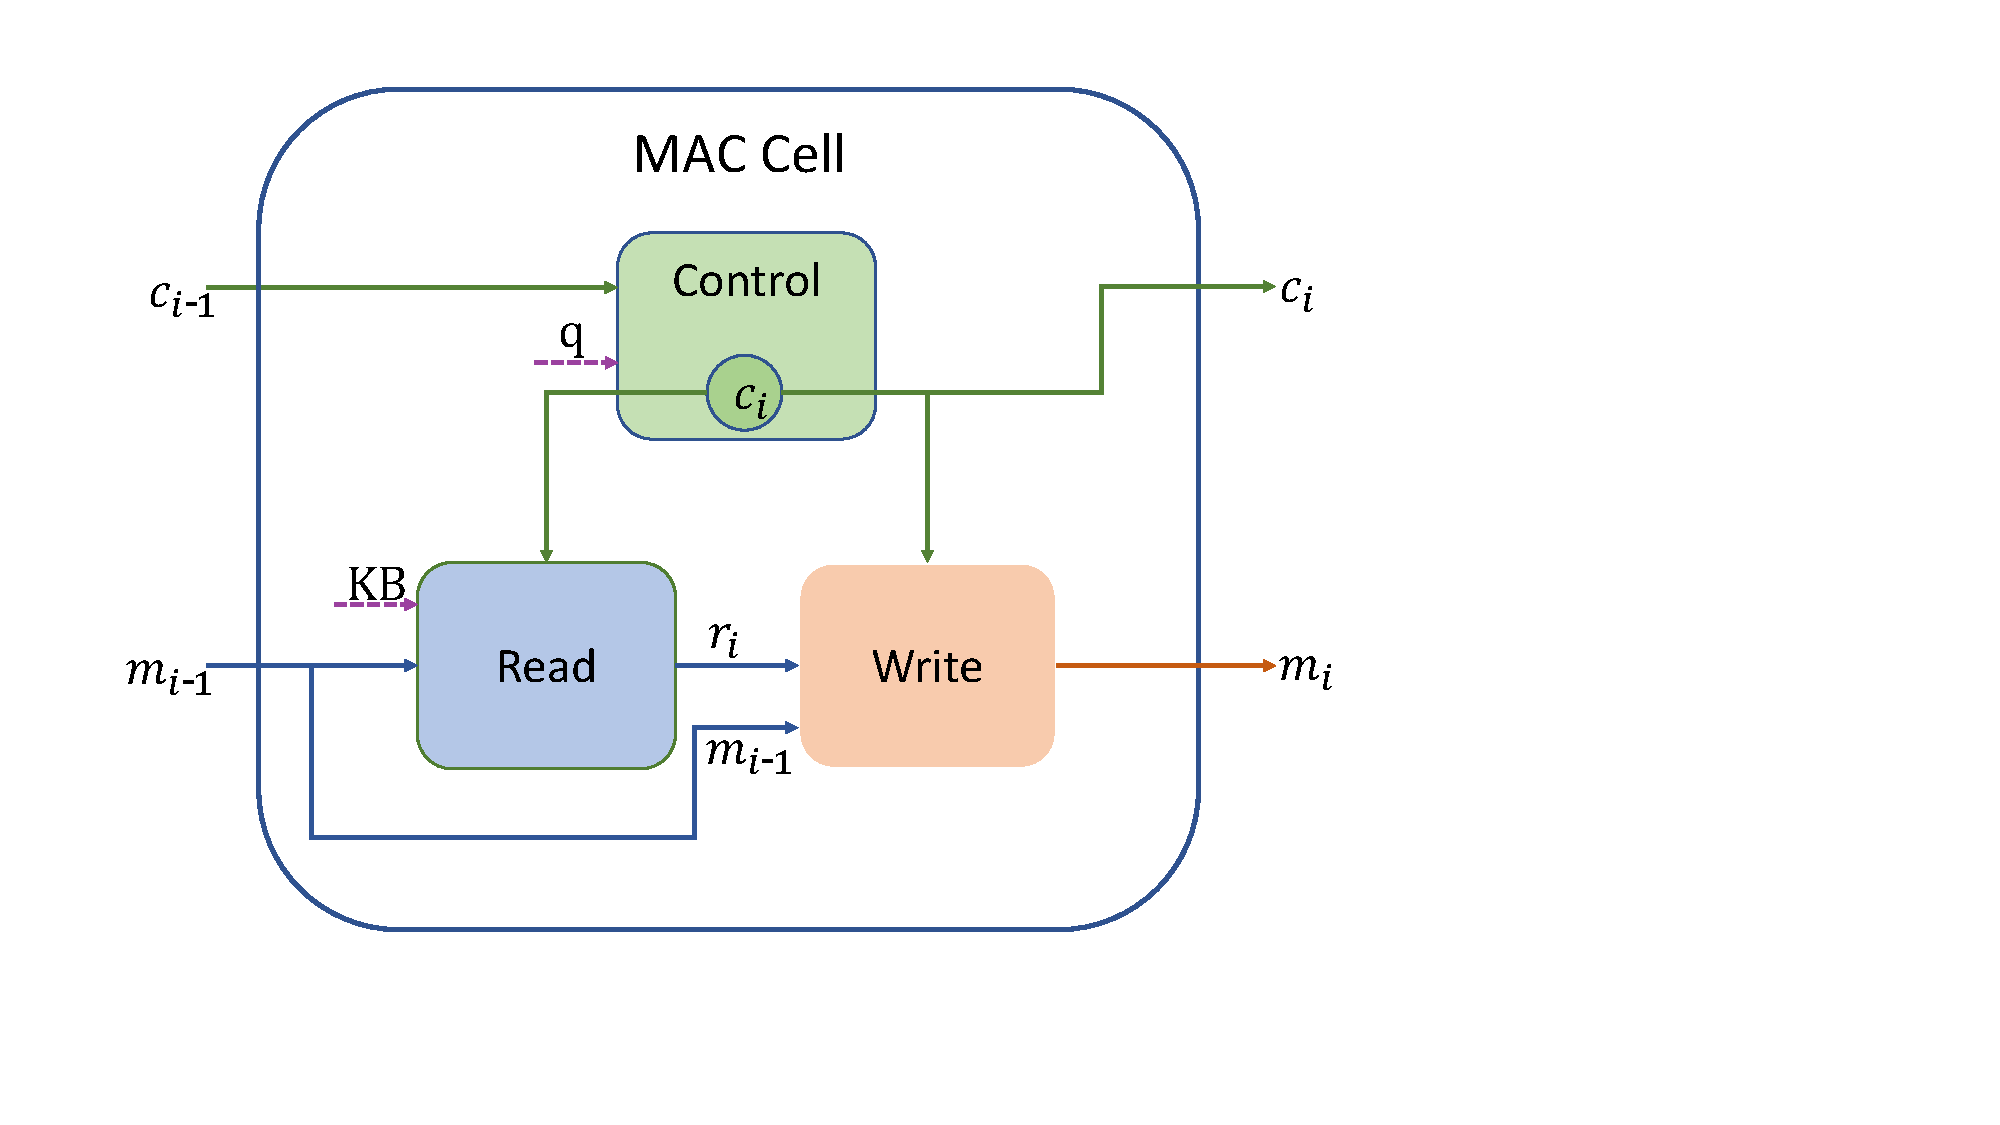
\includegraphics[width=0.7\textwidth]{img/mac_cell.pdf}
	\caption{The Mac Cell. The MAC recurrent cell consists of a control unit, read unit, and write unit, that operate over dual control and memory hidden states. }
	\label{fig:mac_cell}
\end{figure}






